% Magic comments - Informa ao compilador algumas regras de execução, como tipo de compilação ou codificação do texto
% !TeX root = ufop-modelo-trabalho-academico-ichs.tex
% !TeX encoding = UTF-8
% !BIB TS-program = XeLaTex
% !backend = biber
%% abtex2-modelo-trabalho-academico.tex, v-1.9.2 laurocesar
%% Copyright 2012-2014 by abnTeX2 group at http://abntex2.googlecode.com/ 
%%
%% This work may be distributed and/or modified under the
%% conditions of the LaTeX Project Public License, either version 1.3
%% of this license or (at your option) any later version.
%% The latest version of this license is in
%%   http://www.latex-project.org/lppl.txt
%% and version 1.3 or later is part of all distributions of LaTeX
%% version 2005/12/01 or later.
%%
%% This work has the LPPL maintenance status `maintained'.
%% 
%% The Current Maintainer of this work is the abnTeX2 team, led
%% by Lauro César Araujo. Further information are available on 
%% http://abntex2.googlecode.com/
%%
%% This work consists of the files abntex2-modelo-trabalho-academico.tex,
%% delo-include-comandos and abntex2-modelo-references.bib
%%

% ------------------------------------------------------------------------
% ------------------------------------------------------------------------
% abnTeX2: Modelo de trabalho Academico (tese de doutorado, dissertacao de
% mestrado e trabalhos monograficos em geral) em conformidade com 
% ABNT NBR 14724:2011: Informacao e documentacao - Trabalhos academicos -
% Apresentacao
% ------------------------------------------------------------------------
% ------------------------------------------------------------------------

\documentclass[
	% -- opções da classe memoir --
	12pt,				% tamanho da fonte
	openright,			% capítulos começam em pág ímpar (insere página vazia caso preciso)
	twoside,			% para impressão em verso e anverso. Oposto a oneside
	a4paper,			% tamanho do papel. 
	% -- opções da classe abntex2 --
	%chapter=TITLE,		% títulos de capítulos convertidos em letras maiúsculas
	%section=TITLE,		% títulos de seções convertidos em letras maiúsculas
	%subsection=TITLE,	% títulos de subseções convertidos em letras maiúsculas
	%subsubsection=TITLE,% títulos de subsubseções convertidos em letras maiúsculas
	% -- opções do pacote babel --
	english,			% idioma adicional para hifenização
	brazil				% o último idioma é o principal do documento
	]{abntex2ufop} % classe abntex2ufop para escrita de trabalhos academicos

% ---
% Pacotes básicos 
% ---
\usepackage{graphicx}			% Inclusão de gráficos
\usepackage{microtype} 			% para melhorias de justificação
\usepackage{amsmath,amssymb,unicode-math} % escrita matematica
\usepackage{relsize} % readicionado comando \part não funciona. Ver: https://github.com/abntex/abntex2/issues/109
\usepackage{verbatim}

% para incluir páginas pdf diretamente no documento
\usepackage{pdfpages} 
\usepackage{csquotes}
%%%%%%%%%%%%%%%%%%%%%%%%%%%%%%%%%%%%%%%%%%%%%%%%%%%%%%%%%%%%%%%%%%%%%%%%%
% Pacotes de citações: retire o comentário do estilo que deseja usar
%%%%%%%%%%%%%%%%%%%%%%%%%%%%%%%%%%%%%%%%%%%%%%%%%%%%%%%%%%%%%%%%%%%%%%%%%
% Usando o pacote biblatex-abnt e o biber para a compilacao das fontes

% Opção 1: notas de referência, com citações reduzidas (idem, ibidem opcit...)
%\usepackage[backend=biber,style=abnt-ibid,sccite,scbib,justify,extrayear,citecount,noslsn,backref,repeatfields]{biblatex}

% Opção 2: notas explicativas, ou autor-data
\usepackage[backend=biber,
%%%%---configuracoes do estilo abnt
style=abnt,
sccite,
ittitles,
citecount,
scbib,
justify,
noslsn,
repeatfields,		
sorting=nty,
]{biblatex}

\addbibresource{referencias-teste.bib}

% ---
% Personalização do estilo biblatex-abnt
%---
% Adequa as urls de acordo com normas 6023:218:
\DeclareFieldFormat{url}{\bibstring{urlfrom}\addcolon\addspace \url{#1}}%

\DeclareFieldFormat{urldate}{\bibstring{urlseen}\addcolon\addspace #1}%

% Reseta contadores das notas de rodapé em cada capítulo
\makeatletter
\@addtoreset{footnote}{chapter}
\makeatother

% Comandos para exibir uma caixa colorida de fundo cinza para notas historicas
\newcommand{\caixabranca}{\fbox}
\newcommand{\caixa}[1]{\caixabranca{\small{\begin{minipage}{\textwidth-2.5cm}{#1}\end{minipage}}}}

% Pacotes adicionais, usados apenas no âmbito do Modelo Canônico do abnteX2 - pode ser removido
% ---
% Pacotes adicionais, usados no anexo do modelo de folha de identificação
% ---
\usepackage{supertabular}
\usepackage{multicol}
\usepackage{multirow}
\usepackage{lipsum}				% para geração de dummy text
% ---



% ---
% Informações de dados para CAPA e FOLHA DE ROSTO
% ---
\titulo{Modelo de trabalho acad{\^e}mico (monografia, dissertação, tese) com \abnTeX~para estudantes do ICHS-UFOP}
\autor{Estudante}
\local{Mariana}
\data{2019}
\orientador{profa. Marie S. Curie, PhD.}
\coorientador{prof. A. de Saint-Exupéry, PhD.}
\instituicao{Universidade Federal de Ouro Preto - UFOP - Instituto de Ciências Humanas e Sociais - ICHS}
\tipotrabalho{Dissertação de Mestrado}
% O preambulo deve conter o tipo do trabalho, o objetivo, 
% o nome da instituição e a área de concentração 
\preambulo{Trabalho apresentado ao Curso XXX da Universidade Federal de Ouro Preto como parte dos requisitos para a obten{\c c}{\~a}o do Grau de Mestre em XXXX.}
% ---


% ---
% Configurações de aparência do PDF final

% alterando o aspecto da cor azul
\definecolor{blue}{RGB}{41,5,195}

% informações do PDF
\makeatletter
\hypersetup{
     	%pagebackref=true,
		pdftitle={\@title}, 
		pdfauthor={\@author},
    	pdfsubject={\imprimirpreambulo},
	    pdfcreator={LaTeX with abnTeX2},
		pdfkeywords={abnt}{latex}{abntex}{abntex2}{trabalho acadêmico}, 
		colorlinks=true,       		% false: boxed links; true: colored links
    	linkcolor=blue,          	% color of internal links
    	citecolor=blue,        		% color of links to bibliography
    	filecolor=magenta,      		% color of file links
		urlcolor=blue,
		%bookmarksdepth=4
}
\makeatother
% --- 

% --- 
% Espaçamentos entre linhas e parágrafos 
% --- 

% O tamanho do parágrafo é dado por:
\setlength{\parindent}{1.3cm}

% Controle do espaçamento entre um parágrafo e outro:
\setlength{\parskip}{0.2cm}  % tente também \onelineskip

% ---
% compila o indice
% ---
\makeindex
% ---

% ----
% Início do documento
% ----
\begin{document}

% Retira espaço extra obsoleto entre as frases.
\frenchspacing 

% ----------------------------------------------------------
% ELEMENTOS PRÉ-TEXTUAIS
% ----------------------------------------------------------
% \pretextual

% ---
% Capa
% ---
\imprimircapa
% ---

% ---
% Folha de rosto
% (o * indica que haverá a ficha bibliográfica)
% ---
\imprimirfolhaderosto*
% ---


% ---
% Inserir a ficha bibliografica
% ---

% Isto é um exemplo de Ficha Catalográfica, ou ``Dados internacionais de
% catalogação-na-publicação''. 
% Porém, a biblioteca da sua universidade lhe fornecerá um PDF
% com a ficha catalográfica definitiva após a defesa do trabalho. Quando estiver
% com o documento, salve-o como PDF no diretório do seu projeto e substitua todo
% o conteúdo de implementação deste arquivo pelo comando abaixo que está comentado 
% (nao se esqueça de comentar o antigo ambiente de ficha catalográfica):
%
% \begin{fichacatalografica}
%     \includepdf{fig_ficha_catalografica.pdf}
% \end{fichacatalografica}
%
%
% Ou, você poderá também ler os dados da ficha e adicionar no póprio código
% como as palavras-chave, CDU e dimensões do trabalho: 
\begin{fichacatalografica}
	\vspace*{\fill}					% Posição vertical
	\hrule							% Linha horizontal
	\begin{center}					% Minipage Centralizado
	\begin{minipage}[c]{12.5cm}		% Largura
	
	\imprimirautor
	
	\hspace{0.5cm} \imprimirtitulo  / \imprimirautor. --
	\imprimirlocal, \imprimirdata-
	
	\hspace{0.5cm} \pageref{LastPage} p. : il. (algumas color.) ; 30 cm.\\
	
	\hspace{0.5cm} \imprimirorientadorRotulo~\imprimirorientador\\
	
	\hspace{0.5cm}
	\parbox[t]{\textwidth}{\imprimirtipotrabalho~--~\imprimirinstituicao,
	\imprimirdata.}\\
	
	\hspace{0.5cm}
		1. Palavra-chave1.
		2. Palavra-chave2.
		I. Orientador.
		II. Universidade Federal de Ouro Preto.
		III. Instituto de Ciências Humanas e Sociais.
		IV. Título\\ 			
	
	\hspace{8.75cm} CDU 02:141:005.7\\
	
	\end{minipage}
	\end{center}
	\hrule
\end{fichacatalografica}
% ---

% ---
% Inserir folha de aprovação
% ---

% Isto é um exemplo de Folha de aprovação, elemento obrigatório da NBR
% 14724/2011 (seção 4.2.1.3). Você pode utilizar este modelo até a aprovação % do trabalho. Após isso, substitua todo o conteúdo deste arquivo por uma % imagem da página assinada pela banca com o comando abaixo:
%
% \includepdf{folhadeaprovacao_final.pdf}
%
\begin{folhadeaprovacao}
% 
   Dissertação defendida e aprovada, em $XX$ de $XX$ de \imprimirdata, pela comiss{\~a}o avaliadora constitu{\'i}da pelos professores:
   \vspace*{\fill}
   \assinatura{\textbf{\imprimirorientador} \\ Orientador} 
   \vspace*{\fill}
   \assinatura{\textbf{Prof. Oliver Heaviside, Dr.} \\ Convidado}
   \vspace*{\fill}
   \assinatura{\textbf{Prof. William Thomson, Dr.} \\ Convidado}
   \vspace*{\fill}
   %\assinatura{\textbf{Professor} \\ Convidado 3}
  % \vspace*{\fill}
   %\assinatura{\textbf{Professor} \\ Convidado 4}
  % \vspace*{\fill}
      
   \begin{center}
    \vspace*{0.5cm}
    {\large\imprimirlocal}, {\large\imprimirdata}
    \vspace*{1cm}
  \end{center}
  
\end{folhadeaprovacao}
% ---

% ---
% Dedicatória
% ---
\begin{dedicatoria}
   \vspace*{\fill}
   \flushright
   \noindent
   \textit{Matéria é a parte acidental. (Oliver Lodge)} \vspace*{\fill}
\end{dedicatoria}
% ---

% ---
% Agradecimentos
% ---
\begin{agradecimentos}
\noindent Os agradecimentos principais são direcionados à Gerald Weber, Miguel Frasson,
Leslie H. Watter, Bruno Parente Lima, Flávio de Vasconcellos Corrêa, Otavio Real
Salvador, Renato Machnievscz\footnote{Os nomes dos integrantes do primeiro
projeto abn\TeX\ foram extraídos de
\url{http://codigolivre.org.br/projects/abntex/}} e todos aqueles que
contribuíram para que a produção de trabalhos acadêmicos conforme
as normas ABNT com \LaTeX\ fosse possível.

\noindent Agradecimentos especiais são direcionados ao Centro de Pesquisa em Arquitetura
da Informação\footnote{\url{http://www.cpai.unb.br/}} da Universidade de
Brasília (CPAI), ao grupo de usuários
\emph{latex-br}\footnote{\url{http://groups.google.com/group/latex-br}} e aos
novos voluntários do grupo
\emph{\abnTeX}\footnote{\url{http://groups.google.com/group/abntex2} e
\url{http://abntex2.googlecode.com/}}~que contribuíram e que ainda
contribuirão para a evolução do \abnTeX.

\end{agradecimentos}
% ---

% ---
% Epígrafe
% ---
\begin{epigrafe}
    \vspace*{\fill}
	\begin{flushright}
		\textit{``Matéria é a parte acidental.'' (Oliver Lodge)}
	\end{flushright}
\end{epigrafe}
% ---

% ---
% RESUMOS
% ---

% resumo em português
\setlength{\absparsep}{18pt} % ajusta o espaçamento dos parágrafos do resumo
\begin{resumo}
 \noindent O resumo deve ressaltar o objetivo, o método, os resultados e as conclusões do documento. A ordem e a extensão
 destes itens dependem do tipo de resumo (informativo ou indicativo) e do tratamento que cada item recebe no documento original. O resumo deve ser precedido da referência do documento, com exceção do resumo inserido no
 próprio documento. (\ldots) As palavras-chave devem figurar logo abaixo do resumo, antecedidas da expressão Palavras-chave:, separadas entre si por
 ponto e finalizadas também por ponto.

 \textbf{Palavras-chaves}: latex. abntex. editoração de texto.
\end{resumo}

% resumo em inglês
\begin{resumo}[Abstract]
 \begin{otherlanguage*}{english}

\noindent This is the english abstract.

   \vspace{\onelineskip}
 
   \noindent 
   \textbf{Key-words}: latex. abntex. text editoration.
 \end{otherlanguage*}
\end{resumo}

% resumo em francês 
%\begin{resumo}[Résumé]
% \begin{otherlanguage*}{french}
%    Il s'agit d'un résumé en français.
% 
%   \textbf{Mots-clés}: latex. abntex. publication de textes.
% \end{otherlanguage*}
%\end{resumo}
%
%% resumo em espanhol
%\begin{resumo}[Resumen]
% \begin{otherlanguage*}{spanish}
%   Este es el resumen en español.
%  
%   \textbf{Palabras clave}: latex. abntex. publicación de textos.
% \end{otherlanguage*}
%\end{resumo}
%% ---
% ---
% inserir lista de ilustrações
% ---
\pdfbookmark[0]{\listfigurename}{lof}
\listoffigures*
\cleardoublepage
% ---

% ---
% inserir lista de tabelas
% ---
\pdfbookmark[0]{\listtablename}{lot}
\listoftables*
\cleardoublepage
% ---

% ---
% inserir lista de abreviaturas e siglas
% ---
\begin{siglas}
  \item[ABNT] Associação Brasileira de Normas Técnicas
  \item[abnTeX] ABsurdas Normas para TeX
\end{siglas}
% ---

% ---
% inserir lista de símbolos
% ---
\begin{simbolos}
  \item[$ \Gamma $] Letra grega Gama
  \item[$ \Lambda $] Lambda
  \item[$ \zeta $] Letra grega minúscula zeta
  \item[$ \in $] Pertence
\end{simbolos}
% ---

% ---
% inserir o sumario
% ---
\pdfbookmark[0]{\contentsname}{toc}
\tableofcontents*
\cleardoublepage
% ---
% Comando para resetar contadores das notas de rodapé
\makeatletter
\@addtoreset{footnote}{chapter}
\makeatother



% ----------------------------------------------------------
% ELEMENTOS TEXTUAIS
% ----------------------------------------------------------
\textual
% ----------------------------------------------------------
% PARTE
% ----------------------------------------------------------
\part{Preparação da pesquisa}
% ----------------------------------------------------------
%
% ---
% Modelo de capitulo com a introducao, objetivos e estrutura do texto
% ---
% ----------------------------------------------------------
% Introdução (exemplo de capítulo sem numeração, mas presente no Sumário)
% ----------------------------------------------------------
\chapter[Introdução]{Introdução}
%\addcontentsline{toc}{chapter}{Introdução}
% ----------------------------------------------------------

\section{Justificativas e Relev{\^a}ncia}
%
Este documento e seu código-fonte são exemplos de referência de uso da classe
\textsf{abntex2} e do pacote \textsf{biblatex-abnt}. O documento exemplifica uma realização possível entre as opções existentes na norma ABNT NBR 10520:2018 \emph{Citações em documentos -- Apresentação} e da norma ABNT NBR 6023:2018 \emph{Referências -- Elaboração}, cientes de que existe uma distância entre as ``normas'' e a interpretação das normas. Assim, antes de tudo, converse com seu orientador ou representantes do programa de pós-graduação de sua universidade, mostre uma cópia do documento PDF gerado por este arquivo e certifique-se de que não terá problas futuros com relação à aceitação ou não do modelo.

A expressão ``Modelo Canônico'' é utilizada para indicar que \abnTeX\ não é modelo específico de nenhuma universidade ou instituição, mas que implementa tão somente os requisitos das normas da ABNT. 

\section{Metodologia}
Comecemos então com um exemplo de citação, como esta aqui, feita em notas explicativas,\footcite[Esta é uma nota explicativa. Cf. e.g.,][\S 12]{boyle1772} conforme a norma NBR 10520:2018, existem dois tipos de citações em notas de rodapé:
\begin{citacao}
	\begin{itemize}
		\item[$3.6$] \textbf{notas de rodapé:} Indicações, observações ou aditamentos ao texto feitos pelo autor, tradutor ou editor, podendo	também aparecer na margem esquerda ou direita da mancha gráfica. 
		\item[$3.7$] \textbf{notas explicativas:} Notas usadas para comentários, esclarecimentos ou explanações, que não possam ser incluídos no texto.
	\end{itemize} 
\end{citacao}


Uma outra citação nada a ver.\footcite[Esta é uma outra nota explicativa. Ver também ][p.~12]{herao}
%Uma outra citação nada a ver.\cite[Esta é uma outra nota explicativa. Ver também ][p.~12]{herao}. Ver também \cite{boyle1772}

%\caixa{O autor não é obrigado a seguir as notas explicativas com o comando ``footcite'', que gera a essa nota explicativa.\footcite{boyle1772} Pode utilizar o estilo autor-data igualmente, mas deve seguir o mesmo padrão ao longo do texto. Por exemplo, se usar o comando ``cite'', será gerada a entrada \cite{descartes-oeuvres-volx} ou, se quiser apenas o autor, com o comando ``citeauthor'', será gerada a entrada\citeauthor[][12]{descartes-oeuvres-volx}. Ainda, se quiser imprimir apenas a data de referida obra, basta utilizar o comando ``citedate'', que gera a entrada \citedate[55]{descartes-oeuvres-volx}.}

\lipsum[1]

\section{Objetivos}

\lipsum[7]

\lipsum[8]

\section{Organiza{\c c}{\~a}o e estrutura}

\lipsum*[9-11]

\begin{itemize}
\item item;
\item item;
\item item;
\item item;
\end{itemize}

\section{Cronograma}

Esta seção deve constar somente no projeto de monografia. Não deve aparecer na versão final do texto.

% Please add the following required packages to your document preamble:
% \usepackage[table,xcdraw]{xcolor}
% If you use beamer only pass "xcolor=table" option, i.e. \documentclass[xcolor=table]{beamer}

% Please add the following required packages to your document preamble:
% \usepackage[table,xcdraw]{xcolor}
% If you use beamer only pass "xcolor=table" option, i.e. \documentclass[xcolor=table]{beamer}

Um exemplo de cronograma das atividades é proposto na tabela \ref{tab:cronograma}.\footnote{Voc{\^e} pode elaborar também tabelas online, gerando o código em \LaTeX. Após isso, basta copiar e colar o código aqui. Um exemplo de site é o ``Table Generator''\url{http://www.tablesgenerator.com/}.}
  
\begin{table}[h]
\ABNTEXfontereduzida
\caption[Cronograma das atividades]{Cronograma das atividades de elaboração da monografia.}
\label{tab:cronograma}
\begin{minipage}{0.3\textwidth}
    \centering
\begin{tabular}{|l|l|l|l|l|l|l|l|l|l|l|l|l|l|l|l|l|}
\hline
                             & \multicolumn{16}{c|}{Meses}                                                   \\ \hline
Atividades (Etapas)          & 01 & 02 & 03 & 04 & 05 & 06 & 07 & 08 & 09 & 10 & 11 & 12 & 13 & 14 & 15 & 16 \\ \hline
1. Estudo da teoria          & X  & X  & X  & X  & X  &    &    &    &    &    &    &    &    &    &    &    \\ \hline
2. Atualização bibliográfica & X  & X  & X  & X  & X  & X  & X  &    &    &    &    &    &    &    &    &    \\ \hline
3. Seleção de Material       & X  & X  & X  & X  & X  & X  & X  & X  & X  &    &    &    &    &    &    &    \\ \hline
4. Elaboração da monografia  &    &    &    &    & X  & X  & X  & X  & X  & X  & X  & X  & X  & X  & X  &    \\ \hline
5. Elaboração de Artigo      &    &    &    &    &    &    &    &    & X  & X  & X  & X  & X  & X  & X  &    \\ \hline
6. Defesa da monografia      &    &    &    &    &    &    &    &    &    &    &    &    &    &    &    & X  \\ \hline
\end{tabular}
  \end{minipage}
\end{table}
% ---
% Capitulo com exemplos de comandos inseridos de arquivo externo 
% ---
\chapter{Desenvolvimento}
Inserindo uma figura. A figura \ref{fig:308} ilustra algum ponto importante. 
\begin{figure}[!htbp]
	\centering
	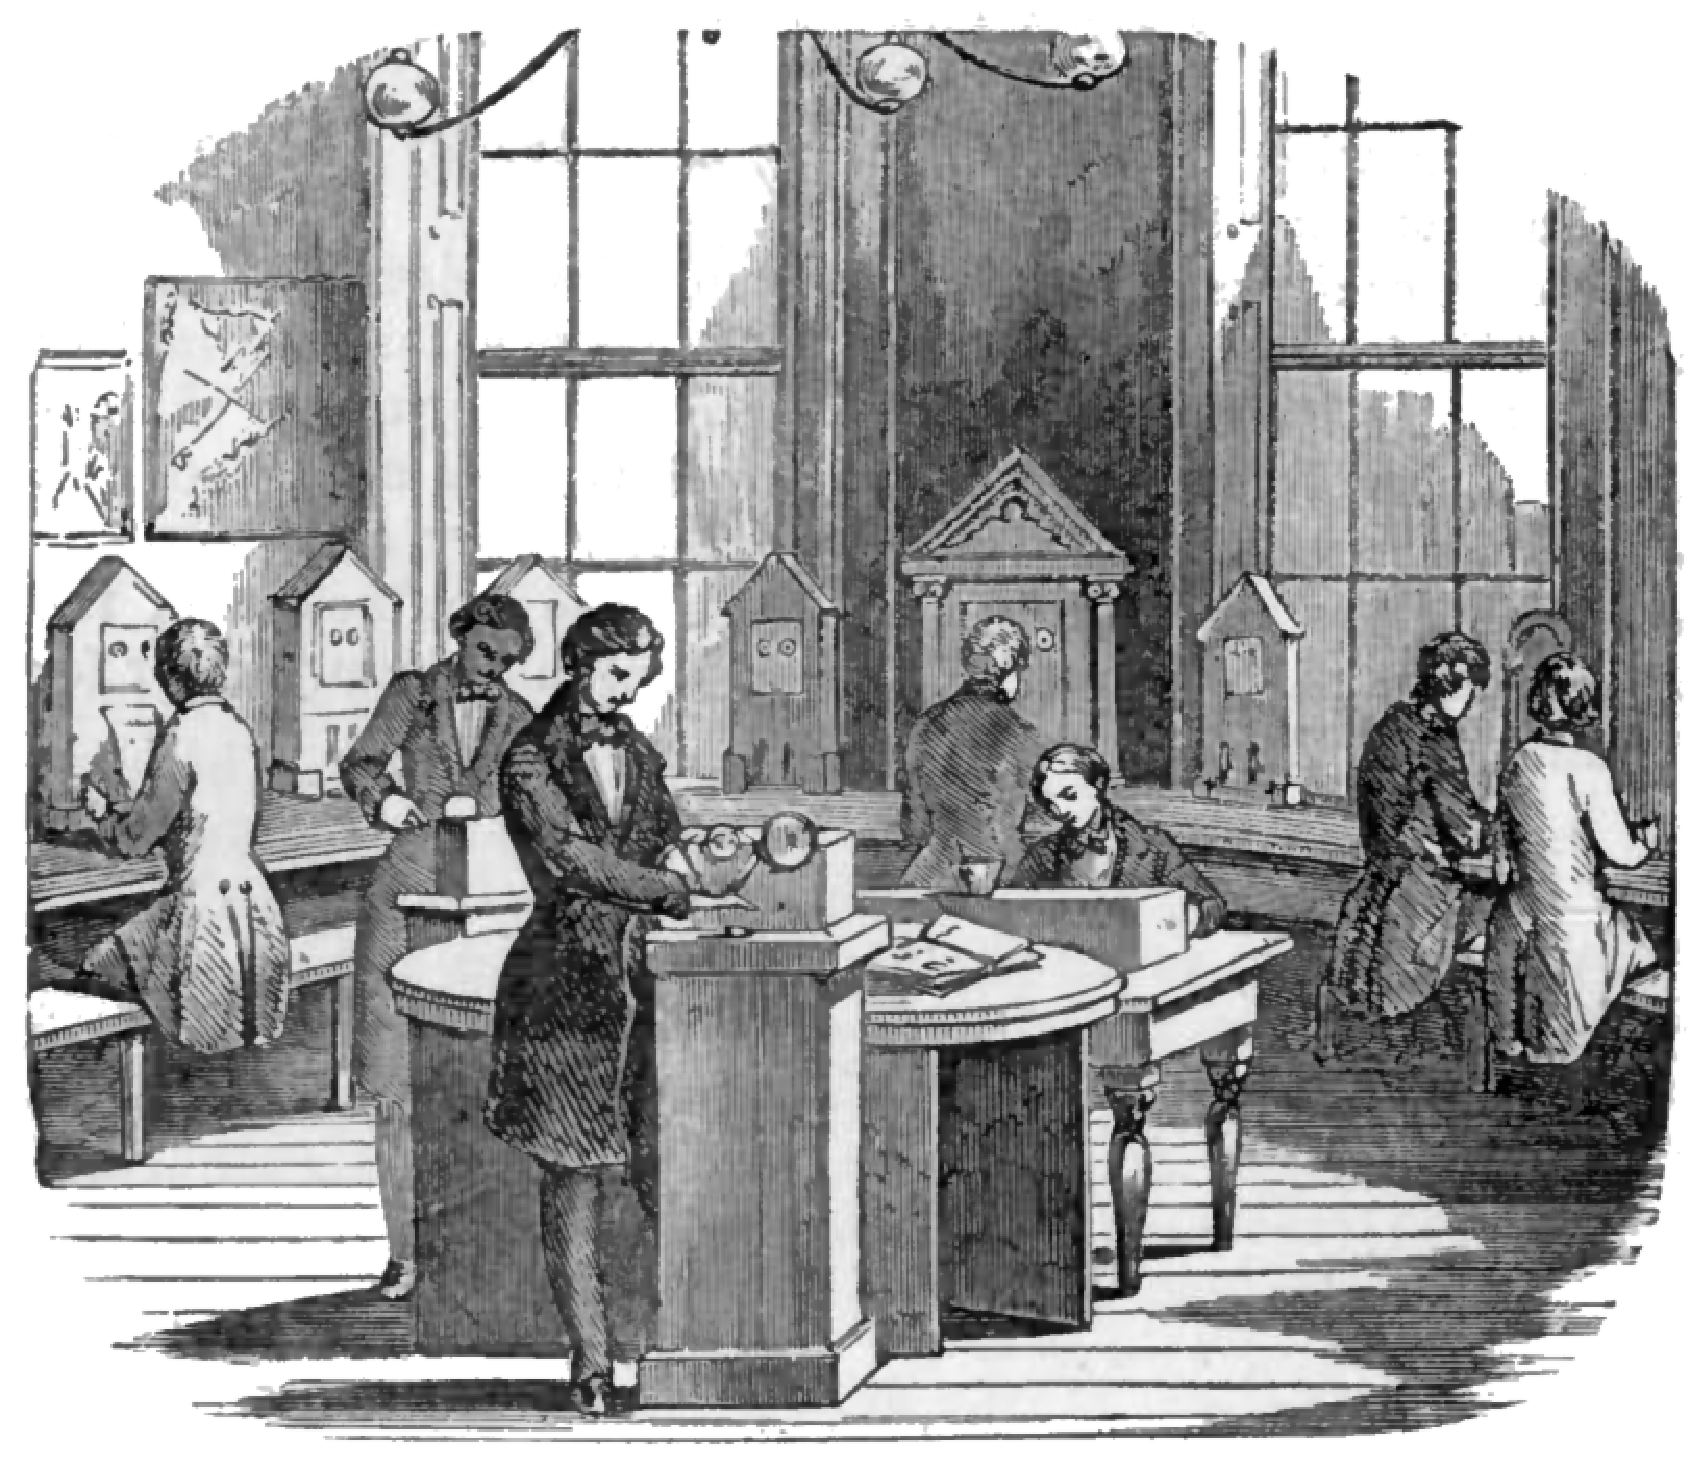
\includegraphics[scale=0.3]{figuras/fig09.pdf} % teste os valores
	\caption[Legenda reduzida - aparece no sumario]{Legenda completa. Aqui você pode colocar uma explicação melhor, sem que ela apareça no sumário do seu trabalho. Fonte: \cite[p.~117]{boyle1772}.} 
	\label{fig:308} 
\end{figure} 

Agora vem uma citação. Segundo Platão, em seu Teeteto:\footcite{platao-teeteto}
\begin{citacao}
	(...) Nam dui ligula, fringilla a, euismod sodales, sollicitudin vel, wisi. Morbi auctor lorem non justo. Nam lacus libero, pretium at, lobortis vitae, ultricies et, tellus. Donec aliquet, tortor sed accumsan bibendum, erat ligula aliquet magna, vitae ornare odio metus a mi. Morbi ac orci et nisl hendrerit mollis. Suspendisse ut massa. Cras nec ante. Pellentesque a nulla. Cum sociis natoque penatibus et magnis dis parturient montes, nascetur ridiculus mus. Aliquam tincidunt urna. Nulla
	ullamcorper vestibulum turpis. Pellentesque cursus luctus mauris.(...)
\end{citacao}

Sendo no ICHS (ver figura \ref{fig:309}, que está na página \pageref{fig:309}), teremos uma noção melhor do movimento estudantil.

\lipsum[30]

\begin{figure}[!htbp]
	\centering
	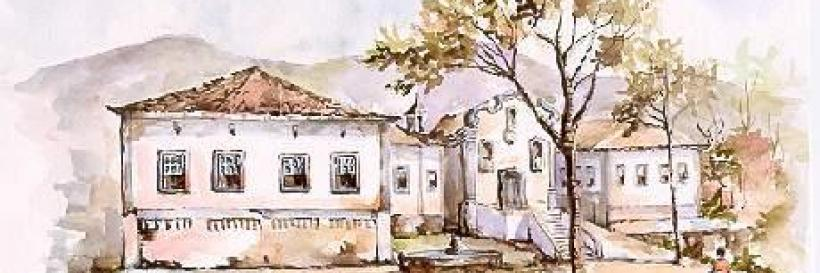
\includegraphics[scale=0.4]{figuras/ichs2.jpg} % teste os valores
	\caption[Legenda reduzida - aparece no sumario]{Legenda completa. Aqui você pode colocar uma explicação melhor, sem que ela apareça no sumário do seu trabalho. Fonte: \cite[p.~117]{boyle1772}.} 
	\label{fig:309} 
\end{figure}
% ---
% ----------------------------------------------------------
% PARTE
% ----------------------------------------------------------
%\part{Referenciais teóricos}
% ----------------------------------------------------------
% ---
% Capitulo de revisão de literatura
% ---
%\chapter{Uma breve hist{\'o}ria da teoria}
% ---

% ---
\section{Uma sec{\c c}{\~a}o}
% ---

\lipsum[1]

\lipsum[2-3]
% ----------------------------------------------------------
% PARTE
% ----------------------------------------------------------
%\part{Resultados}
% ----------------------------------------------------------
% ---
% primeiro capitulo de Resultados
%\chapter{Resultados}
% ---

% ---
\section{Vestibulum ante ipsum primis in faucibus orci luctus et ultrices
posuere cubilia Curae}
% ---

\lipsum[21-22]
% ----------------------------------------------------------
% Finaliza a parte no bookmark do PDF
% para que se inicie o bookmark na raiz
% e adiciona espaço de parte no Sumário
% ----------------------------------------------------------
%\phantompart
% ---
% Insere arquivo de Considerações Finais ou Conclusões
% ---
%\chapter*[Conclusão]{Conclusão}
\addcontentsline{toc}{chapter}{Conclusão}
% ---

\lipsum[31-33]
% ----------------------------------------------------------
% ELEMENTOS PÓS-TEXTUAIS
% ----------------------------------------------------------
\postextual
% ----------------------------------------------------------

%% ----------------------------------------------------------
%% Referências bibliográficas
%% ----------------------------------------------------------
% toca nome de bibliografia para ``Referências''
\printbibliography[title=Refer{\^e}ncias]

% ----------------------------------------------------------
% Glossário
% ----------------------------------------------------------
%
% Consulte o manual da classe abntex2 para orientações sobre o glossário.
%
%\glossary

% ----------------------------------------------------------
% Apêndices
% ----------------------------------------------------------
%(Lembre-se: Apendices são de autoria do próprio autor do texto. 
% Anexos são elementos de autorias de outros, que o autor do texto julga interessante apresentar)
% ---
% Inicia os apêndices: 
% ---
\begin{apendicesenv}

% Imprime uma página indicando o início dos apêndices
\partapendices
% ---
% Insere arquivo com os apendices A e B
% ----------------------------------------------------------
\chapter{Quisque libero justo}
% ----------------------------------------------------------

\lipsum[50]

% ----------------------------------------------------------
\chapter{Nullam elementum urna vel imperdiet sodales elit ipsum pharetra ligula
ac pretium ante justo a nulla curabitur tristique arcu eu metus}
% ----------------------------------------------------------
\lipsum[55-57]
\end{apendicesenv}
% ---

% ----------------------------------------------------------
% Anexos
% ----------------------------------------------------------
%(Lembre-se: Apendices são de autoria do próprio autor do texto. 
% Anexos são elementos de autorias de outros, que o autor do texto julga interessante apresentar)
% ---
% Inicia os anexos
% ---
\begin{anexosenv}

% Imprime uma página indicando o início dos anexos
\partanexos

% ---
% Insere arquivo com os anexos 1, 2 e 3
\chapter{Morbi ultrices rutrum lorem.}
% ---
\lipsum[30]

% ---
\chapter{Cras non urna sed feugiat cum sociis natoque penatibus et magnis dis
parturient montes nascetur ridiculus mus}
% ---

\lipsum[31]

% ---
\chapter{Fusce facilisis lacinia dui}
% ---

\lipsum[32]

% ---
\end{anexosenv}

%---------------------------------------------------------------------
% INDICE REMISSIVO
%---------------------------------------------------------------------
%\phantompart
\printindex
%---------------------------------------------------------------------

\end{document}
